% Author: Izaak Neutelings (September 2020)
\documentclass[border=3pt,tikz]{standalone}
\usepackage{amsmath}
\usepackage{tikz}
\usepackage{physics}
\usepackage[outline]{contour} % glow around text
\usetikzlibrary{calc}
\usetikzlibrary{decorations.markings}
\usetikzlibrary{angles,quotes} % for pic
\usetikzlibrary{arrows.meta} % for arrow size
\usetikzlibrary{bending} % for arrow head angle
\usetikzlibrary{decorations.pathmorphing} % for decorate random steps
\tikzset{>=latex} % for LaTeX arrow head
\usepackage{xcolor}
\contourlength{1.3pt}

\colorlet{xcol}{blue!70!black}
\colorlet{xcol'}{xcol!50!red}
\colorlet{vcol}{green!45!black}
\colorlet{acol}{red!50!blue!80!black!80}
\tikzstyle{rvec}=[->,very thick,xcol,line cap=round]
\tikzstyle{vvec}=[->,very thick,vcol,line cap=round]
\tikzstyle{avec}=[->,very thick,acol,line cap=round]
\colorlet{myred}{red!65!black}
\tikzstyle{force}=[->,myred,very thick,line cap=round]
\tikzstyle{mass}=[line width=0.5,draw=red!50!black,fill=red!50!black!10,rounded corners=1,
                  top color=red!50!black!30,bottom color=red!50!black!10,shading angle=20]
\tikzstyle{disk}=[line width=0.5,orange!30!black,fill=orange!40!black!10,
                  top color=orange!40!black!20,bottom color=orange!40!black!10,shading angle=20]
\tikzstyle{pole}=[line width=0.5,blue!20!black,fill=orange!20!black!10,
                  top color=blue!20!black!20,bottom color=blue!20!black!10,shading angle=20]
\tikzstyle{rope}=[brown!70!black,line width=1,line cap=round] %very thick
\tikzstyle{myarr}=[-{Latex[length=3,width=2,flex'=1]},thin]
\tikzstyle{mydashed}=[dash pattern=on 2pt off 1pt]
\def\rope#1{ \draw[rope,black,line width=1.4] #1; \draw[rope,line width=1.1] #1; }
\def\tick#1#2{\draw[thick] (#1) ++ (#2:0.1) --++ (#2-180:0.2)}
\newcommand\rightAngle[4]{
  \pgfmathanglebetweenpoints{\pgfpointanchor{#2}{center}}{\pgfpointanchor{#3}{center}}
  \coordinate (tmpRA) at ($(#2)+(\pgfmathresult+45:#4)$);
  %\draw[white,line width=0.6] ($(#2)!(tmpRA)!(#1)$) -- (tmpRA) -- ($(#2)!(tmpRA)!(#3)$);
  \draw[black] ($(#2)!(tmpRA)!(#1)$) -- (tmpRA) -- ($(#2)!(tmpRA)!(#3)$);
}


\begin{document}


% ROTATION
\def\L{3.1}     % axis lengths
\def\R{1.0*\L}  % position vector radial distance
\def\Rang{52}   % position vector angle
\def\ang{25}    % angle of the CM velocity
\begin{tikzpicture}
  \coordinate (O) at (0,0);
  \coordinate (X) at (1.05*\L,0);
  \coordinate (Y) at (0,1.05*\L);
  \coordinate (X') at (\ang:\L);
  \coordinate (Y') at (90+\ang:\L);
  \coordinate (R) at (\Rang:\R);
  \node[fill=blue!40!black,circle,inner sep=0.9] (R') at (R) {};
  \node[above right=-1] at (R') {P};
  \coordinate (Rx) at (0:{\R*cos(\Rang)});
  \coordinate (Ry) at (90:{\R*sin(\Rang)}); %($(Y)!(O)!(R)$);
  \coordinate (Rx') at (\ang:{\R*cos(\Rang-\ang)});
  \coordinate (Ry') at (90+\ang:{\R*sin(\Rang-\ang)});
  
  % AXES
  \draw[<->,very thick,xcol!70!black]
    (X) node[right=-1,xcol] {$x$} -- (O) node[below left=-3] {O} --
    (Y) node[left=-1,xcol] {$y$};
  \draw[<->,very thick,xcol'!70!black]
    (X') node[above=2,right=-2,xcol'] {$x'$} -- (O) --
    (Y') node[left=-2,xcol'] {$y'$};
  
  % POSITION VECTOR
  \draw[rvec,vvec,line cap=round] (O) -- (R') node[midway,left=2,above=1] {$\vb{r}$};
  \draw pic[-{Latex[length=3,width=2,flex'=1]},"$\theta=\omega t$"{scale=0.95,above=2,right},
            draw,angle radius=20,angle eccentricity=1] {angle=X--O--X'};
  
  % ANGLES
  \begin{scope}[xcol!70!black]
    \draw[dashed] (Ry) -- (R') -- (Rx);
    \tick{Rx}{90};
    \tick{Ry}{0};
    \rightAngle{R'}{Rx}{X}{0.25}
    \rightAngle{Y}{Ry}{R'}{0.25}
  \end{scope}
  \begin{scope}[xcol'!70!black]
    \draw[dashed] (Ry') -- (R') -- (Rx');
    \tick{Rx'}{90+\ang};
    \tick{Ry'}{\ang};
    \rightAngle{X'}{Rx'}{R'}{0.25}
    \rightAngle{Y'}{Ry'}{R'}{0.25}
  \end{scope}
  
\end{tikzpicture}


% ROTATION + angles
\begin{tikzpicture}
  \coordinate (Rx'') at (\ang:{\R*cos(\Rang)*cos(\ang)});     % projection of Rx on x' axis
  \coordinate (Ry'') at (90+\ang:{\R*sin(\Rang)*cos(\ang)});  % projection of Ry on y' axis
  \coordinate (Rx''') at ($(R')+(-90+\ang:{\R*sin(\Rang)*cos(\ang)})$); % projection of Rx on R-Rx' line
  \coordinate (Ry''') at ($(R')+(180+\ang:{\R*cos(\Rang)*cos(\ang)})$); % projection of Ry on R-Ry' linex
  
  % TRIANGLES
  \fill[xcol!70!black!10]
    (O) -- (Rx) -- (Rx'') -- cycle
    (O) -- (Ry) -- (Ry'') -- cycle;
  \fill[xcol'!70!black!10]
    (R) -- (Rx) -- (Rx''') -- cycle
    (R) -- (Ry) -- (Ry''') -- cycle;
  \node[fill=blue!40!black,circle,inner sep=0.9] at (R') {};
  \node[above right=-1] at (R') {P};
  
  % AXES
  \draw[<->,very thick,xcol!70!black]
    (X) node[right=-1,xcol] {$x$} -- (O) node[left=1,below=-1] {O} --
    (Y) node[left=-1,xcol] {$y$};
  \draw[<->,very thick,xcol'!70!black]
    (X') node[above=2,right=-2,xcol'] {$x'$} -- (O) --
    (Y') node[left=-2,xcol'] {$y'$};
  
  % POSITION VECTOR
  \draw[vvec,line cap=round] (O) -- (R'); %node[midway,left=2,above=1] {$\vb{r}$};
  \draw pic["$\theta$"{scale=0.9},
            draw,angle radius=20,angle eccentricity=1.22] {angle=X--O--X'};
  \draw pic["$\theta$"{scale=0.9},
            draw,angle radius=20,angle eccentricity=1.22] {angle=Y--O--Y'};
  \draw pic["$\theta$"{scale=0.9},
            draw,angle radius=17,angle eccentricity=1.30] {angle=Rx--R'--Rx'};
  \draw pic["$\theta$"{scale=0.9},
            draw,angle radius=17,angle eccentricity=1.30] {angle=Ry--R'--Ry'};
  
  % ANGLES
  \begin{scope}[xcol!80!black]
    \draw[dashed]
      (Ry) -- (R') node[midway,above=-1,scale=0.9] {$x$} --
      (Rx) node[midway,left=-1,scale=0.9] {$y$};
    \tick{Rx}{90};
    \tick{Ry}{0};
    \rightAngle{R'}{Rx}{X}{0.25}
    \rightAngle{Y}{Ry}{R'}{0.25}
  \end{scope}
  \begin{scope}[xcol'!80!black]
    \draw[dashed] (Ry') -- (R') -- (Rx''');
    \draw[dashed] (Ry) -- (Ry'');
    \draw[dashed] (Rx) -- (Rx'');
    \draw[dashed] (Rx) -- (Rx''');
    \draw[dashed] (Ry) -- (Ry''');
    \tick{Rx'}{90+\ang};
    \tick{Ry'}{\ang};
    \tick{Rx''}{90+\ang};
    \tick{Ry''}{\ang};
    \rightAngle{X'}{Rx'}{R'}{0.25}
    \rightAngle{Y'}{Ry'}{R'}{0.25}
    \rightAngle{Rx}{Rx''}{O}{0.25}
    \rightAngle{Ry}{Ry''}{O}{0.25}
    \rightAngle{Ry}{Ry'''}{R}{0.25}
    \rightAngle{Rx}{Rx'''}{R}{0.25}
  \end{scope}
  
  % LENGTHS
  %\node[xcol!70!black,above,scale=0.8] at ($(Ry)!0.5!(R)$) {$x$};
  \node[xcol!80!black!60,above,scale=0.8,rotate=\ang] at ($(O)!0.6!(Rx'')$) {$x\cos\theta$};
  \node[xcol'!80!black!60,right=1,below=-2,scale=0.8,rotate=\ang] at ($(Rx)!0.6!(Rx''')$) {\contour{white}{$y\sin\theta$}};
  %\node[xcol!80!black!60,below=4,scale=0.8,rotate=-90+\ang] at ($(O)!0.6!(Ry'')$) {$y\cos\theta$};
  \node[xcol'!80!black!60,below=-1,scale=0.8,rotate=-90+\ang] at ($(Ry)!0.6!(Ry''')$) {\contour{white}{$x\sin\theta$}};
  \draw[<->,xcol!80!black!60]
    ([shift={(180+\ang:0.3)}]O) -- ([shift={(180+\ang:0.3)}]Ry'')
    node[xcol!80!black!60,midway,scale=0.8,rotate=-90+\ang,fill=white,inner sep=0.5] {$y\cos\theta$};
  
\end{tikzpicture}



% STATIONARY REFERENCE FRAME - CENTRIFUGAL
\def\R{2}      % disk radius
\def\t{0.1}    % disk thickness
\def\p{0.05}   % pole radius
\def\P{1.3}    % pole height
\def\r{0.24}   % mass radius
\def\L{0.7*\R} % rope length
\def\H{2.0}    % human height
\begin{tikzpicture}
  
  % PERSON
  \coordinate (H) at (0,\H);
  \draw[thick,line cap=round]
    (H)++(-165:0.3) to[out=-140,in=60]++ (-130:0.3)
    to[out=65,in=-90,looseness=1.0]++ (80:0.45) to[out=90,in=120,looseness=1.4]++ (20:0.2); % pony tail
  \draw[thick,fill=white] (H) circle (0.3);
  \draw[thick,line cap=round] (H)++(-140:0.3) to[out=80,in=-120,looseness=1.8]++ (40:0.6); % hair
  \draw[thick] (H)++(-90:0.3) coordinate (N) to[out=-95,in=95]++ (0,-0.40*\H) coordinate (P);
  \draw[thick,line cap=round] (N)++(-95:0.03) to[out=-60,in=95]++ (0.10*\H,-0.4*\H) coordinate (RH);
  \draw[thick,line cap=round] (N)++(-95:0.03) to[out=-120,in=90]++ (-0.08*\H,-0.4*\H);
  \draw[thick] (P) to[out=-70,in=95] (0.08*\H,0);
  \draw[thick] (P) to[out=-100,in=72] (-0.06*\H,0);
  
  % AXIS
  \node (A) at (0.38*\H,0.94*\H) {S};
  \draw[<->,line width=0.9]
    (A)++(0.25*\H,0.28*\H) node[left,scale=0.9] {$z$} --++ (0,-0.3*\H) coordinate (O) --++
         (0.3*\H,0) node[below right=-3.5,scale=0.9] {$y$};
  \draw[->,line width=0.9] (O) --++ (-120:0.25*\H) node[left=-2,scale=0.9] {$x$};
  
  % DISK
  \begin{scope}[shift={(0.5*\H+\R,0.3*\H)}]
    \coordinate (T) at (0,\r);
    \draw[disk] (-\R,0) --++ (0,-\t) arc(180:360:{\R} and {0.4*\R}) --++ (0,\t);
    \draw[disk] (0,0) ellipse({\R} and {0.4*\R});
    \rope {(T) --++ (\L,0) coordinate (M)};
    \draw[pole] (-\p,\P) --++ (0,-\P) arc(180:360:{\p} and {0.4*\p}) --++ (0,\P);
    \draw[pole] (0,\P) ellipse({\p} and {0.4*\p});
    \rope {(-1.4*\p,0.85*\r) arc(180:360:{1.4*\p} and {0.4*\p})}
    \rope {(-1.4*\p,1.00*\r) arc(180:360:{1.4*\p} and {0.4*\p})}
    \rope {(-1.4*\p,1.15*\r) arc(180:360:{1.4*\p} and {0.4*\p})}
    \draw[force] (M)++(150:1.1*\r) --++ (-0.5*\L,0) node[above=-1] {$\vb{T}$};
    \draw[avec] (M)++(210:1.1*\r) --++ (-0.5*\L,0) node[right=0,below=-1] {$\vb{a}$}; %_\mathrm{cm}
    \draw[mass] (M) circle(\r) node {$m$};
    \draw[->] (10:1.05*\R) arc(10:50:{1.05*\R} and {0.4*\R}) node[above left=-2] {$\omega$};
    \draw[vvec] (0,\P+0.014) --++ (0,0.7*\L) node[midway,left] {$\vb*\omega$};
  \end{scope}
  
\end{tikzpicture}


% MOVING REFERENCE FRAME - CENTRIFUGAL
\begin{tikzpicture}
  
  % DISK
  \coordinate (T) at (0,\r);
  \draw[disk] (-\R,0) --++ (0,-\t) arc(180:360:{\R} and {0.4*\R}) --++ (0,\t);
  \draw[disk] (0,0) ellipse({\R} and {0.4*\R});
  
  % PERSON
  \draw[thick,fill=white] (-0.35*\R,\H) circle (0.15*\H) coordinate (H);
  \draw[thick] (H)++(-90:0.15*\H) coordinate (N) to[out=-95,in=95]++ (0,-0.40*\H) coordinate (P);
  \draw[thick,line cap=round] (N)++(-95:0.03) to[out=-70,in=190]++ (0.34*\H,-0.20*\H);
  \draw[thick,line cap=round] (N)++(-95:0.03) to[out=-120,in=-80]++ (-0.17*\H,-0.12*\H) to[out=100,in=-100]++ (0.02*\H,0.25*\H);
  \draw[thick] (P) to[out=-70,in=95] ($(H)+(0.08*\H,-\H)$);
  \draw[thick] (P) to[out=-100,in=72] ($(H)+(-0.08*\H,-\H)$);
  
  % POLE + MASS
  \rope {(T) --++ (\L,0) coordinate (M)};
  \draw[pole] (-\p,\P) --++ (0,-\P) arc(180:360:{\p} and {0.4*\p}) --++ (0,\P);
  \draw[pole] (0,\P) ellipse({\p} and {0.4*\p});
  \rope {(-1.4*\p,0.85*\r) arc(180:360:{1.4*\p} and {0.4*\p})}
  \rope {(-1.4*\p,1.00*\r) arc(180:360:{1.4*\p} and {0.4*\p})}
  \rope {(-1.4*\p,1.15*\r) arc(180:360:{1.4*\p} and {0.4*\p})}
  \draw[force] (M)++(150:1.1*\r) --++ (-0.5*\L,0) node[above=-1] {$\vb{T}$};
  \draw[force] (M)++(30:1.1*\r) --++ (0.5*\L,0) node[above=0] {$\vb{F}_\mathrm{cf}$};
  \draw[mass] (M) circle(\r) node {$m$};
  
  % AXIS
  \node (A) at (57:0.88*\R) {S$'$};
  \draw[<->,line width=0.9]
    (A)++(0.25*\H,0.28*\H) node[left,scale=0.9] {$z'$} --++ (0,-0.3*\H) coordinate (O) --++
         (0.3*\H,0) node[below right=-3.5,scale=0.9] {$y'$};
  \draw[->,line width=0.9] (O) --++ (-120:0.25*\H) node[left=-2,scale=0.9] {$x'$};
  
\end{tikzpicture}


% STATIONARY REFERENCE FRAME - CORIOLIS
\def\R{2}       % disk radius
\def\r{0.1}     % mass radius
\def\v{0.35*\R} % mass velocity
\def\x{0.48}    % mass position (fraction of \R)
\def\ang{50}    % angle displacement
\begin{tikzpicture}
  \coordinate (O) at (0,0);
  \coordinate (T) at (0,\r);
  \coordinate (M) at (90:0.45*\R);
  \coordinate (S) at (-145:1.6*\R);
  \coordinate (B) at (90+\x*\ang:0.88*\R);
  
  % DISK & DOTS
  \draw[disk] (O) circle(\R);
  \fill[myred!20] (90:0.88*\R) circle(0.05*\R);
  \fill[myred] (90+\x*\ang:0.88*\R) circle(0.05*\R);
  \fill[myred!20] (90+\ang:0.88*\R) circle(0.05*\R);
  \draw[xcol,->] (92:0.88*\R) arc(92:88+\ang:0.88*\R);
  
  % MASS
  \draw[<->,black!25,line width=0.9]
    (0,0.35*\R) |-++ (0.35*\R,-0.35*\R);
  \draw[xcol] (O) --++ (90:1.1*\R);
  \draw[vvec] (M) --++ (90:\v) node[below right] {$\vb{v}$};
  \draw[mass] (M) circle(\r) node[right=1] {$m$};
  \draw[->] (10:1.1*\R) arc(10:35:1.1*\R) node[left=2,above=0] {$\omega$};
  
  % AXIS
  \node[left=2] at (S) {S};
  \draw[<->,line width=0.9]
    (S)++(0,0.38*\R) node[left,scale=0.9] {$y$} |-++
         (0.35*\R,-0.35*\R) node[below right=-3,scale=0.9] {$x$};
  
  % AXIS S'
  \draw[<->,line width=0.9]
    (90+\x*\ang:0.35*\R) node[below left=-2,scale=0.9] {$y'$} -- (0,0) --
    (\x*\ang:0.35*\R) node[above=3,right=-2,scale=0.9] {$x'$};
  \node[below=1] at (O) {A};
  \node[right=1,below=1] at (B) {B};
  
\end{tikzpicture}


% MOVING REFERENCE FRAME - CORIOLIS
\begin{tikzpicture}
  \def\v{0.40*\R}        % mass velocity
  \def\vv{2.0}           % velocity for plot
  \def\FC{0.30*\R}       % Coriolis force
  \def\om{180/pi}        % angular frequency omega
  \def\tmax{1.10}        % maximum t
  \def\xt{0.98*\x*\tmax} % mass position
  \coordinate (T) at (0,\r);
  \coordinate (S) at (-145-\ang:1.6*\R);
  \coordinate (M) at ({\vv*\xt*sin(\om*\xt)},{\vv*\xt*cos(\om*\xt)});
  \coordinate (V) at ({\v*sin(\om*\xt)+\v*\xt*cos(\om*\xt)},{\v*cos(\om*\xt)-\v*\xt*sin(\om*\xt)});
  \coordinate (F) at ({\FC*cos(\om*\xt)-\FC*\xt*sin(\om*\xt)},{-\FC*sin(\om*\xt)-\FC*\xt*cos(\om*\xt)});
  
  % DISK & DOTS
  \draw[disk] (0,0) circle(\R);
  \fill[myred] (90:0.88*\R) circle(0.05*\R);
  
  % AXIS
  \draw[xcol,dashed] (0,0) --++ (90:1.1*\R);
  \node[below left=-1] at (0,0) {S$'$};
  \draw[<->,line width=0.9]
    (0,0.35*\R) node[left,scale=0.9] {$y'$} |-++
    (0.35*\R,-0.35*\R) node[below right=-3.5,scale=0.9] {$x'$};
  
  % MASS
  \draw[xcol,samples=50,smooth,variable=\t,domain=0:\tmax]
    plot({\vv*\t*sin(\om*\t)},{\vv*\t*cos(\om*\t)});
  %\fill[myred] (90-\ang:0.88*\R) circle(0.05); % check
  \draw[vvec] (M) --++ (V) node[above=3,left=0] {$\vb{v}$};
  \draw[force] (M) --++ (F) node[right=-1] {$\vb{F}_\mathrm{Cor}$};
  \draw[mass] (M) circle(\r) node[left=4,above=2] {$m$};
  
  % AXIS
  \node[left=2] at (S) {S};
  \draw[<->,black!25,line width=0.9]
    (-145:1.6*\R)++(0,0.38*\R) node[left,scale=0.9] {$y$} |-++
                   (0.35*\R,-0.35*\R) node[below right=-3,scale=0.9] {$x$};
  \draw[<->,line width=0.9]
    (S)++(90-\ang:0.38*\R) node[left=3,scale=0.9] {$y$} --++ (-90-\ang:0.38*\R) --++
         (-\ang:0.38*\R) node[below right=-3,scale=0.9] {$x$};
  \draw[->] (-165:1.55*\R) arc(-150:-210:0.6*\R) node[midway,left=0] {$\omega$};
  
\end{tikzpicture}


% CENTRIFUGAL + CORIOLIS
\begin{tikzpicture}
  \def\vv{3.2}         % velocity for plot
  \def\v{0.25*\R}      % velocity size
  \def\Fc{0.40*\R}     % centrifugal force
  \def\FC{0.30*\R}     % Coriolis force
  \def\om{180/pi}      % angular frequency omega
  \def\tmax{1.6}       % maximum t
  \def\ta{0.26*\tmax} % mass position A
  \def\tb{0.60*\tmax} % mass position B
  \def\tc{0.90*\tmax} % mass position C
  \def\vRM#1{{\vv*#1*sin(\om*#1)},{\vv*#1*cos(\om*#1)}}
  \def\vvc#1{{\v*sin(\om*#1)+\v*#1*cos(\om*#1)},{\v*cos(\om*#1)-\v*#1*sin(\om*#1)}}
  \def\vFc#1{{\Fc*#1*sin(\om*#1)},{\Fc*#1*cos(\om*#1)}}
  \def\vFC#1{{\FC*cos(\om*#1)-\FC*#1*sin(\om*#1)},{-\FC*sin(\om*#1)-\FC*#1*cos(\om*#1)}}
  \def\vang#1{atan2({\v*cos(\om*#1)-\v*#1*sin(\om*#1)},{\v*sin(\om*#1)+\v*#1*cos(\om*#1)})}
  \coordinate (O) at (0,0);
  \coordinate (MA) at (\vRM{\ta});
  \coordinate (MB) at (\vRM{\tb});
  \coordinate (MC) at (\vRM{\tc});
  %\node[mass,circle,inner sep=2] (MA) at (\vRM{\ta}) {};
  %\node[mass,circle,inner sep=2] (MB) at (\vRM{\tb}) {};
  %\node[mass,circle,inner sep=2] (MC) at (\vRM{\tc}) {};
  
  % AXIS
  \node[below left=-1] at (0,0) {S$'$};
  \draw[<->,line width=0.9]
    (0,0.5*\R) node[left,scale=0.9] {$y'$} |-++
    (0.5*\R,-0.5*\R) node[below right=-3.5,scale=0.9] {$x'$};
  
  % PLOT
  \draw[xcol,samples=50,smooth,variable=\t,domain=0:\tmax]
    plot({\vv*\t*sin(\om*\t)},{\vv*\t*cos(\om*\t)});
  \draw[dashed,xcol] (O) -- (MA);
  \draw[dashed,xcol] (O) -- (MB);
  \draw[dashed,xcol] (O) -- (MC);
  
  % MASS A
  \draw[vvec]  (MA)++({\vang{\ta}}:\r) --++ (\vvc{\ta}) node[right=1,above=-2] {$\vb{v}$};
  \draw[force] (MA)++(90-\om*\ta:\r) --++ (\vFc{\ta}) node[above=3,left=0] {$\vb{F}_\mathrm{cf}$};
  \draw[force] (MA)++({\vang{\ta}-90}:\r) --++ (\vFC{\ta}) node[right=6,below=-1] {\contour{white}{$\vb{F}_\mathrm{Cor}$}};
  \draw[mass]  (MA) circle(\r); %node[left=4,above=2] {$m$};
  
  % MASS B
  \draw[vvec]  (MB)++({\vang{\tb}}:\r) --++ (\vvc{\tb}) node[right=-2] {$\vb{v}$};
  \draw[force] (MB)++(90-\om*\tb:\r) --++ (\vFc{\tb}) node[above=3,left=3] {$\vb{F}_\mathrm{cf}$};
  \draw[force] (MB)++({\vang{\tb}-90}:\r) --++ (\vFC{\tb}) node[right=4,below=-2] {$\vb{F}_\mathrm{Cor}$};
  \draw[mass]  (MB) circle(\r);
  
  % MASS C
  \draw[vvec]  (MC)++({\vang{\tc}}:\r) --++ (\vvc{\tc}) node[right=-2] {$\vb{v}$};
  \draw[force] (MC)++(90-\om*\tc:\r) --++ (\vFc{\tc}) node[above=-1] {$\vb{F}_\mathrm{cf}$};
  \draw[force] (MC)++({\vang{\tc}-90}:\r) --++ (\vFC{\tc}) node[below=2,left=-5] {$\vb{F}_\mathrm{Cor}$};
  \draw[mass]  (MC) circle(\r);
  
\end{tikzpicture}


% EARTH + CENTRIFUGAL
\contourlength{0.7pt}
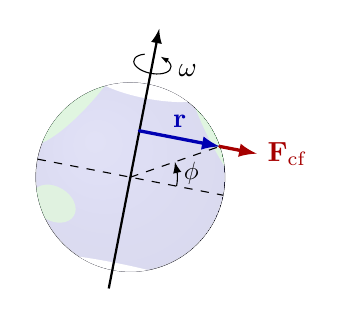
\begin{tikzpicture}
  \def\E{1.2}
  \def\ang{30} % latidude
  \coordinate (O) at (0,0);
  
  % EARTH
  %\draw[dashed,rotate=-11] (0,-1.3*\E) -- (0,1.45*\E);
  \fill[blue!70!black!70] (0,0) circle (1.2);
  \draw[very thin,ball color=blue!70!black!40,fill opacity=0.2] (0,0) circle (\E);
  \begin{scope}[rotate=-11]
    \draw[-{Latex[length=3,width=2,flex'=1]}]
      (0,1.22*\E)++(120:{0.2*\E} and 0.1*\E) arc(120:430:{0.2*\E} and 0.1*\E)
      node[pos=0.7,right=0] {$\omega$};
    \clip (0,0) circle (\E);
    \fill[white] (0,\E) ellipse ({0.6*\E} and {0.15*\E});
    \fill[white] (0,-\E) ellipse ({0.8*\E} and {0.08*\E});
    \fill[green!70!black!60,rotate=-30] (160:1.1*\E) ellipse ({0.2*\E} and {0.8*\E});
    \fill[green!70!black!60,rotate=40] (-10:1.14*\E) ellipse ({0.2*\E} and {0.9*\E});
    \fill[green!60!black!60,very thick,rotate=-20] % Australia
      (230:0.86*\E) ellipse ({0.25*\E} and {0.18*\E});
    \fill[fill=white,fill opacity=0.8] (0,0) circle (\E);
  \end{scope}
  \begin{scope}[rotate=-11]
    %\draw[dashed] (-\E,0) to[out=-20,in=-160] (\E,0);
    %\draw[->,thick] (-1.2*\E,0) -- (1.2*\E,0);
    \draw[dashed] (-\E,0) -- (\E,0) coordinate (X);
    \draw[dashed] (O) -- (\ang:\E) coordinate (R);
    \draw[->,thick] (0,-1.2*\E) -- (0,1.6*\E);
    \draw[rvec] (0,{\E*sin(\ang)}) -- (R) node[midway,above=0] {$\vb{r}$};
    \draw[force] (R) --++ (0.4*\E,0) node[right] {$\vb{F}_\mathrm{cf}$};
    \draw pic[->,"$\phi$"{scale=0.9}, %{Latex[length=3,width=2,flex'=1]}
              draw,angle radius=17,angle eccentricity=1.3] {angle=X--O--R};
  \end{scope}
  
\end{tikzpicture}


% EARTH + CORIOLIS
\contourlength{0.7pt}
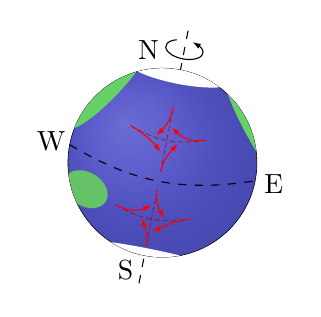
\begin{tikzpicture}
  \def\E{1.2}
  \coordinate (O) at (0,0);
  
  % EARTH
  \draw[dashed,rotate=-11] (0,-1.3*\E) -- (0,1.45*\E);
  \fill[blue!70!black!70] (0,0) circle (1.2);
  \draw[very thin,ball color=blue!70!black!40,fill opacity=0.2] (0,0) circle (\E);
  \begin{scope}[rotate=-11]
    \draw[-{Latex[length=3,width=2,flex'=1]}] (0,1.22*\E)++(120:{0.2*\E} and 0.1*\E) arc(120:430:{0.2*\E} and 0.1*\E);
    \clip (0,0) circle (\E);
    \fill[white] (0,\E) ellipse ({0.6*\E} and {0.15*\E});
    \fill[white] (0,-\E) ellipse ({0.8*\E} and {0.08*\E});
    \fill[green!70!black!60,rotate=-30] (160:1.1*\E) ellipse ({0.2*\E} and {0.8*\E});
    \fill[green!70!black!60,rotate=40] (-10:1.14*\E) ellipse ({0.2*\E} and {0.9*\E});
    \fill[green!60!black!60,very thick,rotate=-20] % Australia
      (230:0.86*\E) ellipse ({0.25*\E} and {0.18*\E});
    \draw[dashed] (-\E,0) to[out=-20,in=-160] (\E,0);
    
    % CORIOLIS
    \draw[myred,mydashed,very thin] (0,-0.1*\E) coordinate (NS) --++ (0, 0.70*\E) coordinate (NN);
    \draw[myred,mydashed,very thin] (0,-0.3*\E) coordinate (SN) --++ (0,-0.60*\E) coordinate (SS);
    \draw[myred,mydashed,very thin] (-0.4*\E,0.32*\E) coordinate (NW) to[out=-20,in=-160]++ (0.8*\E,0) coordinate (NE);
    \draw[myred,mydashed,very thin] (-0.4*\E,-0.53*\E) coordinate (SW) to[out=-20,in=-160]++ (0.8*\E,0) coordinate (SE);
    \draw[myarr,red] (NN) to[out=-90,in=  50]++ (-110:0.35*\E); % northern hemisphere
    \draw[myarr,red] (NS) to[out= 90,in=-120]++ (  70:0.35*\E);
    \draw[myarr,red] (SN) to[out=-90,in= 130]++ ( -65:0.30*\E); % southern hemisphere
    \draw[myarr,red] (SS) to[out= 90,in= -60]++ ( 110:0.30*\E);
    \draw[myarr,red] (NE) to[out=200,in= -40]++ (170:0.38*\E); % northern hemisphere
    \draw[myarr,red] (NW) to[out=-20,in= 140]++ (-30:0.42*\E);
    \draw[myarr,red] (SE) to[out=200,in=  40]++ (210:0.42*\E); % southern hemisphere
    \draw[myarr,red] (SW) to[out=-20,in=-140]++ ( 10:0.38*\E);
  \end{scope}
  
  \node at (108-11:1.2*\E) {N};
  \node at (180-11:1.2*\E) {W};
  \node at (   -11:1.2*\E) {E};
  \node at (-98-11:1.2*\E) {S};
  
\end{tikzpicture}


\end{document}